\documentclass[letterpaper,11pt,titlepage]{article}
\usepackage{epsfig,xspace,url}
\usepackage{authblk}
\usepackage[margin=.5in]{geometry}
\usepackage{setspace}
\doublespace

\iffalse 
\addtolength{\oddsidemargin}{-.25in}
\addtolength{\evensidemargin}{-.25in}
\addtolength{\textwidth}{.5in}

\addtolength{\topmargin}{-.25in}
\addtolength{\textheight}{1in}

\fi

\title{Linear Approximation of Shortest Common Superstrings}
\author[1]{Sarah Spall and Scott Bauer}

\begin{document}
\maketitle
\newpage

\subsection*{Introduction}
A superstring of a set of strings $S$, is a string $w$, such that each string $s \in S$ is a substring
of $w$.  The goal of shortest common superstring (SCS) problem is to find the shortest possible $w$, such that each 
string $s \in S$ is a substring of $w$. This problem has found application in both DNA sequencing 
and data compression.  DNA is made up of four neucleotides, {A, C, G, and T}.  Sequencing molecules also known as,
determining a ``string'' over the alphabet of neucleotides, is an important part of biology. In practice, biochemist use SCS to sequence molecules, by finding the SCS for the fragments.

The optimization version of this problem has been shown to be NP-hard \cite{blum1991linear} \cite{gallant1980finding}, 
so research has focused on finding approximation algorithms.  The first approximation 
algorithm was a greedy algorithm discussed in Gallant (1982). This algorithm because a commonly used approximation algorithm and is newer papers.  The GREEDY algorithm works for a set of strings $S$ by finding two strings $s,t \in S$, that have maximum overlap.  The overlap string is formed from $s$ and $t$, and  is placed back in $S$.  Strings $s$ and $t$ are then removed from $S$.  This process is repeated until
$S$ contains one string, or there is no non-empty overlap between strings in $S$.  This algorithm is later
addressed in \cite{turner1989approximation}, \cite{tarhio1988greedy}, \cite{li1990towards}, and \cite{blum1991linear}.
\cite{tarhio1988greedy} developed an algorithm implementing the greedy approximation, and conjectured that 
the length of the superstring produced by the GREEDY algorithm is less than or equal to $2*len(OPT)$, where $OPT$ is the length of the optimal shortest common superstring of $S$.  They were unable
to prove the upper bound, and it remained an open problem.  \cite{turner1989approximation} was also unable to prove
the conjectured $2*len(OPT)$ upper bound of the greedy approximation.  The first proven bound was from Li (1990) \cite{li1990towards}, who showed an upper bound of $O(n\log n)$, on an approximation algorithm for the shortest common superstring, where $n$ is the length of the optimal solution. Blum et al. \cite{blum1991linear} was then the first to prove a $O(n)$ bound, with a modified version of the commonly used greedy algorithm, and was also able to prove a $4*n$ upper bound on the length of the superstring produced by the greedy approximation algorithm.  Now we will go into more detail about previous work on the shortest common superstring problem. 

\subsection*{Notational preliminaries}

Let $S = \{s_1 \ldots, s_m\}$ be a set of $m$ strings over the alphabet $\sum$. The paper uses $OPT(S)$ to denote the length of the shortest common superstring for the set $S$. The overlap of two strings, $s$ and $t$ is $v$ where $s=uv$ and $t=vw$. The length of this overlap $v$ is denoted $ov(s,t) = |v|$. The prefix of a string $s$ with respect to $t$, is $u$, where $s=uv$ and $t=vw$. The prefix of $s$ with respect to $t$ is denoted by $pref(s,t)$. The distance between a string $s$ and a string $t$ is denoted by $d(s,t)$ and is equal to $|u| = |pref(s,t)|$. There are these notions $first(SCS)$ and $last(SCS)$ which denote the first string in $SCS$ is the first string in the set $S$, and $last(SCS)$ is the last string in $SCS$. That is $first(SCS) = s_1$ and $last(SCS) = s_m$.

\newpage

\textbf{Distance graph}
The graph $G = (V,E,d)$ is an edge-weighted, complete directed graph. The set of vertices $V$ is the set of strings $S$. That is each vertex in $V$ is one of the strings $\{s_1, ..., s_m\} \in S$. The weight is denoted $d(v_i,v_j)$ where $d(v_i,v_j)$ is equal to $d(s_i,s_j)$. The weights of edges is the distance between strings $s_i$ and $s_j$. Lastly, $E=V^2$.

\begin{figure}[h]
 \centering
   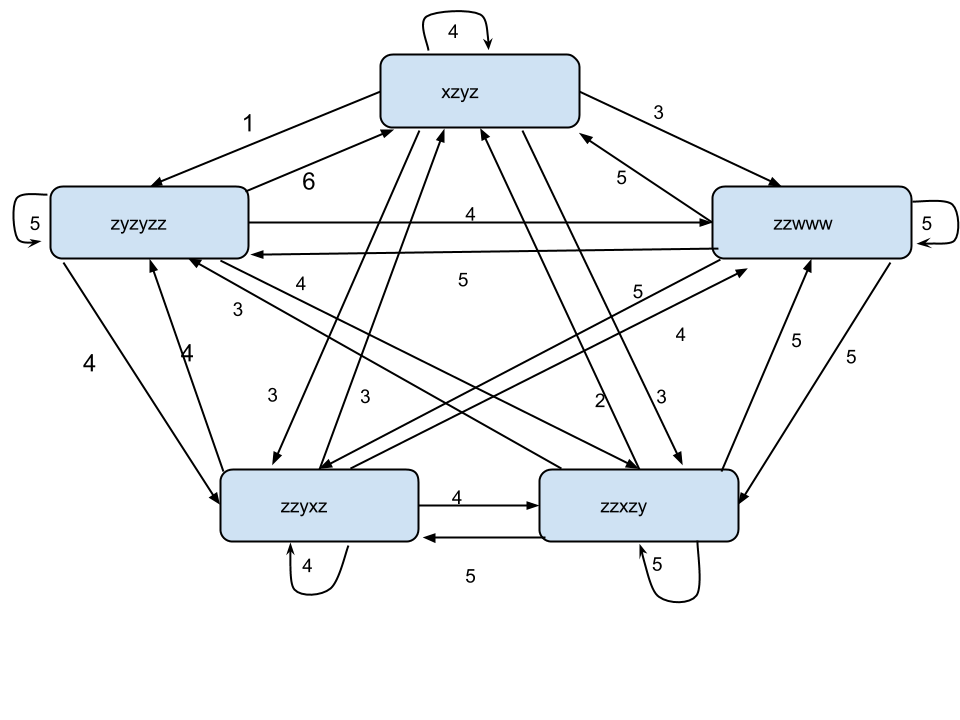
\includegraphics[width=.6\textwidth]{distance.png}
\end{figure}


\textbf{Overlap graph}
The graph $G = (V,E,ov)$ is an edge-weighted, complete directed graph. Just as the distance graph, $V \in S$ and $E=V^2$. The weight of edges in the overlap graph is the length of the overlap between strings $s_i$ and $s_j$, ie $ov(s_i,s_j)$. 

\begin{figure}[h]
 \centering
   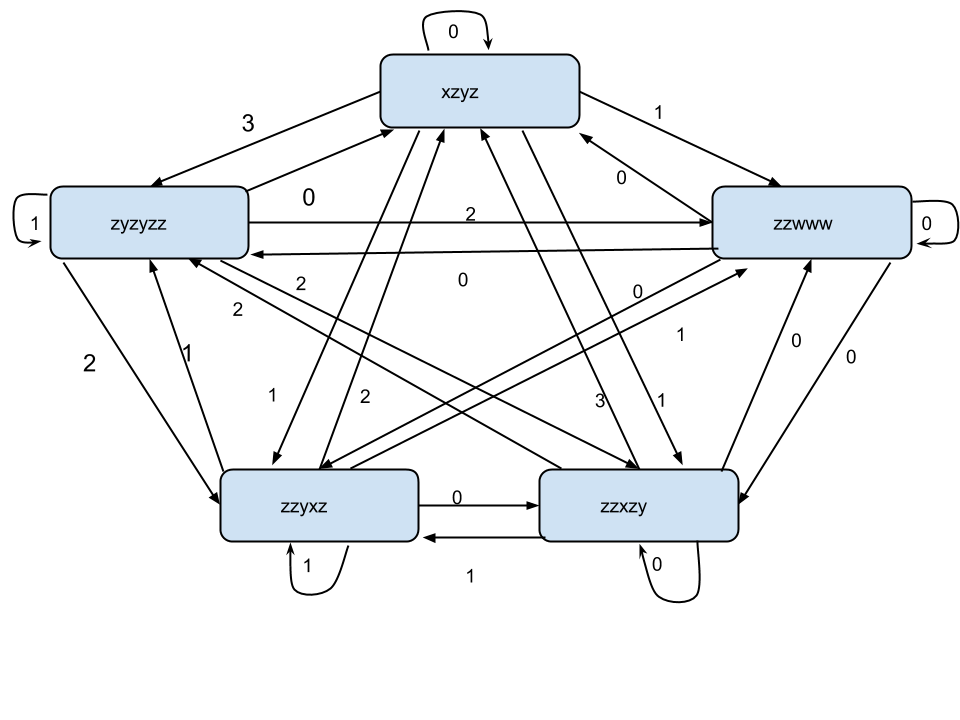
\includegraphics[width=.6\textwidth]{overlap.png}
\end{figure}


\newpage
\subsection*{Related Work}

Blum et al. and prior work on the SCS problem has focused on finding approximation algorithms because SCS was first shown to be NP-hard in 1977. And again in 1980 by Gallant et al. \textit{On Finding Minimal length superstrings}\cite{gallant1980finding}.  Gallant et al., proved that given an unbounded alphabet $\sum$, a positive length $K$, and a set of strings $S$ over $\sum$, that determining if $S$ has a superstring of length $K$ is NP-Complete.


 The authors do this by reducing to the \textit{Hamiltonian  path problem}. The Hamiltonian path problem is the problem where one determines in a directed or undirected graph whether there exists a path that visits each vertex only once. The Hamiltonian path problem was known to be NP-Complete so a reduction ultimately proves the completeness of the other problem \cite{michael1979computers}. Throughout all newer papers on the SCS problem each paper reduces the problem to the Hamiltonian path problem while using different tricks to reduce the SCS.\\

In \textit{Towards a DNA Sequencing Theory} (1990) \cite{li1990towards}, Ming Li explains the relevance of SCS in terms of DNA sequencing. The idea of sequencing DNA is an important one to understand the basis of life. Cures for diseases, viruses, among other things all come from information that is derived from sequencing DNA.  Biochemists can sequence the DNA of a molecule by using an SCS approximation algorithm on the fragments of the moledules DNA.  Using the SCS problem on DNA was very relevant in the early 90's due to the limited technology of sequencing DNA, and when only around 500 base pairs could be sequenced at a time. Li provides an algorithm in which he proves an approximation algorithm for SCS constructs a superstring of length $O(nlogn)$ where n is the smallest possible superstring. This was the first provably good upper bound with respect to the length of the approximation and the optimal solution.  The algorithm provided in the paper takes the base greedy approximation algorithm, but instead of greedily choosing two strings which have the greatest overlap, the algorithm chooses two strings such that their merge will make it so every other group of strings has some overlap. In simpler terms he tries to maximize the amount of groups a string will overlap with. He calls this technique group merging.

Tarhio and Ukkonen (1988) developed a ``greedy'' approximation algorithm based on an idea first mentioned in Gallant 1982; Find the two strings in a set of strings with the largest overlap and merge these two strings together to form a new overlapped string.  Then add the the new overlapped string to the set of strings and remove two original strings.  Continue to do this until there is only one string in the set.  The main result of this paper dealt with the quality of the approximation, where compression is the measure of quality.  They show that if $n$ is the sum of the length of every string in a set $S$, and $OPT(S)$ is length of the shortest common superstring for $S$, and $k_{greedy}$ is the length of the string produced by their greedy approximation algorithm, then $(n - k_{greedy}) \geq \frac{1}{2}*(n - OPT(S))$.  There is another way to compare the quality of an approximation algorithm for the SCS problem, compare the length of the common superstring created by the approximation, for a set of strings $S$, to the length of $OPT(S)$ for the set of strings $S$.  Tarhio and Ukkonen were unable to prove an upper bound for this quality measure, but conjectured that their approximation algorithm produced common superstrings  of length no more than $2$ times $OPT(S)$; $k_{greedy} \leq 2*k_{min}$.

All work was considered on a reduced set of strings, meaning no string in a set $S$ is a common superstring of another string in $S$, because a reduced set of strings will have the same substring as the non-reduced set.

The SCS problem can be viewed as a special case of the longest Hamiltonian path problem on a weighted directed graph. An approximation solution for SCS was approached as finding the longest Hamiltonian path in a weighted directed graph by more than one paper \cite{tarhio1988greedy} \cite{turner1989approximation}. The definition of overlap, as defined in ``preliminary notation'',  is asymmetric, an overlap between $s_i$ and $s_j$ does not mean there is an overlap between $s_j$ and $s_i$;  an overlap is maximal if it is as large as possible. 

Tarhio defines an ``overlap'' graph $G$ for a set of strings $S = \{s_1, ... ,s_n\}$, with vertex set $S \cup {x_o, x_{n+1}}$, and with directed edges $(s_i, s_j)$, if $s_i \neq s_j$;  $x_o$ is a start node; and $x_{n+1}$ is an end node.  each edge $(s_i, s_j)$ has weight $ov(s_i, s_j)$.  The weight of the edge from $x_o$ to each other vertex is $0$, and the weight from $x_{n+1}$ to every other vertex is $0$.  So, the ``overlap'' graph, is a graph $G = (V, E, ov)$.  From any directed Hamiltonian path $H$ on $G$ from $x_o$ to $x_{n+1}$, a common superstring can be constructed for $S$.  The SCS for $S$ would be constructed then from the longest hamiltonina path on $G$. Since finding the longest Hamiltonian path is NP-hard an approximation algorithm is needed, and there is a well known ``greedy'' heuristic for longest Hamiltonian paths.  To construct a Hamiltonian path, select an edge $e$ from the remaining edges in $G$, the overlap graph, such that $e$ has the largest weight and $e$ plus the edges already selected form a sub graph that can be expanded to a Hamiltonian path.  This is repeated until a Hamiltonian path has been found.  Tarhio used this ``greedy'' approximation algorithm as part of his approximation algorithm for SCS.

Tarhio approached the problem of an approximation algorithm for SCS by reducing the problem to the longest Hamiltonian path problem and using a well known greedy approximation algorithm for longest Hamiltonian path to generate a common superstring. He also gave a guaranteed bound with regards to ``compression'',  and conjectured  that their approximation algorithm produces strings of length less than or equal to $2$ times the length of the $OPT(S)$.  

Another slightly later paper Turner (1989) \cite{turner1989approximation} approached an approximation algorithm for SCS, as Tarhio did, thinking about it from the viewpoint of maximizing the overlap between the strings in a set $S$.  Just as Tarhio, Turner could find no worse example than $k_{greedy} \leq 2* k_{min}$, but was also not able to prove the upper bound.  Turner also showed $(n - k_{greedy}) \geq \frac{1}{2}*(n - OPT(S))$. 

Turner models the problem of finding the SCS as the longest path problem, on a complete directed graph with each edge have a non-negative weight, where the weight is the overlap between strings $s_i$ and $s_j$,the same overlap graph considered by Tarhio et al.  In this specific case of the Longest Path Problem, the goal is to find a Hamiltonian path that maximizes the sum of the weights of the edges of the path. 
Three different approximation algorithms for SCS are then presented in the paper. The first approximation algorithm finds a maximum matching in the overlap graph $G$.  Since $G$ is complete, any matching can be extended to a path, and can be used to find a Hamiltonian path.  This is similar to the approach of Tarhio, except instead of using the ``greedy'' approximation algorithm for longest Hamiltonian paths, he used maximum matchings to construct Hamiltonian paths.  Turner's second approximation algorithm found a directed matching in the overlap graph $G$ which was also used to find a Hamiltonian path.  For his third approximation algorithm Turner proposes the same approximation algorithm as Tarhio and Ukonnen. At the very end of the paper Turner relates SCS to the path version of the traveling salesman problem; This is similar to what is done in Blum et al. 


\subsection*{Main Results}

\subsection*{$4 \ldots OPT(S)$ upper bound for MGREEDY}

Reducing the SCS problem to a weighted directed  graph G, we end up with a set of strings $S$ which can be represented as a distance graph. Doing so opens the potential of finding a common superstring using existing solutions for Hamiltonian path problems. The algorithm works by finding a vertex disjoint cycle cover, where each vertex in the graph is contained in one cycle. In order to get a vertex disjoint cycle cover, the authors use a polynomial-time algorithm for the assignment problem. The assignment problem is the problem of finding a maximal or minimal weight matching between vertices in a weighted bipartite graph. To prove that the algorithm finds a SCS of length at most $4 * OPT(S)$ they prove that the the assignment algorithm finds some optimal weight matching on graph $G$. When the cycles in $G$ are found and unraveled they are at most length 4 of the optimal solution. To prove MGREEDY's approximation they first prove that an algorithm ``Concat-cycles'' produces a string at most 4 of the optimal, then show that MGREEDY mimics concat-cycles.

\textbf{Concat-cycle algorithm}\\

\textbf{A.} Given a set of strings $S$ reduce the set of strings to a distance graph $G$. \\
\textbf{B.} Run a minimum weight assignment on $G$. The resulting set of cycles is $C$ where $C = \{c_1, ..., c_n\}$\\
\textbf{C.} For each cycle $c_i \in C$,  ``unravel'' the cycle into strings $Ps_i'$. $s_i'$ can be defined as the vertices $v_1 ... v_r ... v_1$. This means that $s_i$ represents the  string that is created by traveling through the vertices in a cycle until we've visited ever vertex in that cycle.\\
\textbf{D.} Now, for each string that we created from cycles, concatenate them together which results in a superstring.\\

\textbf{Theorem}
The algorithm concat cycles produces a string of length at most $4 * OPT(S)$\\

\textbf{Explanation of the proof}\\

The proof works by stating that since an optimal assignment on the distance graph $G$ produces a set of cycles $C$, if we sum the weight of the cycles it is less than or equal to OPT(S). That is $C = {c_1, ..., c_m}$ then $\sum_{i=i}^m w(c_i) \leq OPT(S)$. This makes sense because the weights of the edges are just $|s_i| - ov(s_i,s_j)$. That is, the weight of the edge from $v_i$ to $v_j$ is just the length of $s_i$ minus the overlap it has with $s_j$. We will show that the sum of these is less or equal to $OPT(S)$.

The algorithm takes the longest string $l_i$ from the cycle $c_i$ and merges it with all the other longest strings in each cycle. We end up with overlap between strings at most $2*\sum_{i=0}^m w_i$. When the algorithm finishes merging all strings together we have a resulting string with a minimal length of $\sum_{i=1}^m l_i - 2wi$.  They show that $OPT(S)$ is greater than or equal to the two previous summations. When they unroll the cycles and get a string $s'$ they show that $|s'| \leq \sum_{i=1}^m l_i + w+i$. When you do a replacement in the equation you get, $\sum_{i=1}^m l_i + 2w_i + \sum_{i=1}^m 3wi$ which when we replace again: $\leq OPT(S) + 3 * OPT(S) = 4 * OPT(S)$\\

We will explain now how the paper shows that the MGREEDY algorithm mimics concat-cycles and thus has the same upper bound SCS length.

Unlike Concat-cycles, MGREEDY operates on the overlap graph $G$, rather than the distance graph, and computes the maximum overlap. The algorithm works by repeatedly selecting an edge from a list of sorted edges, from highest to lowest. And deciding for each edge whether or not to include it. The algorithm continues by constructing and joining paths until disjoint cycles emerge such that all vertices in $G$ are covered. That is it selects an edge between vertices and merges them into one vertex. The assignment of covers $C$ is an optimal assignment, which they prove through a contradiction. They say that if there exists an edge with a maximum overlap it would have to be contained in the algorithms $C$. Since this is an optimal assignment it mimics the concat-cycles which also creates an optimal assignment. Once the assignment is complete they simply unroll the cycles and concatenate strings together. 

\subsection*{$3 \ldots OPT(S)$ upper bound for TGREEDY}

In the modified GREEDY algorithm the final step was to simply concatenate strings until only one string remained, the SCS. The authors propose that simply concatenating the strings is what is limiting the algorithm. They propose instead of simply concatenating strings together you run the original GREEDY algorithm on the strings. \\

\textbf{Theorem}\\
TGREEDY produces a superstring of at most $3 \ldots OPT(S)$\\

\textbf{Explanation of the proof}

The proof works by taking a set of ``self overlapping'' strings $S$ that were obtained by running MGREEDY, and an assignment $C$. They then create a new set of strings $S'$ which is a set of strings obtained by arbitrarily selecting strings out of a cycle $c_x$, where $x \in S$ and $c_x$ is the cycle corresponding to $x$. With this new set, $S'$ they then create another set $S''$ because they love three levels on indirection, and hate clarity. $S''$ is the set of strings from $S'$ placed into an equivalence class and rotated by one. It turns out $S''$ is a superstring for $S$. They point out that $S' \subseteq S$. From here they calculate some weights of edges in cycles between these prime and double prime sets and use some results from two other papers and get an upper bound of $3n$.\\


\textbf{The superstring problem is MAX SNP-hard}

As the final result of the paper the authors show that the superstring problem is MAX SNP-hard, by reducing TSP(1,2) to the superstring problem; TSP(1,2) was shown to be MAX SNP-hard in \cite{papadimitriou1993}.  Which, although published after Blum et al. was cited by Blum et al. that TSP(1,2) had been shown to be MAX SNP-hard.  MAX SNP is a class of optimization problems, and it is known that every problem in this class can be approximated within some constant factor. 

TSP(1,2) is the special case of the traveling salesman problem where the distances are either $1$ or $2$.  The instance of TSP(1,2) considered in this paper is the instance where each edge in the graph $H$ has distance $1$, and each edge not in the graph has distance $2$.  There is the additional restriction that $H$ have a bounded degree $D$ (the precise bound is not important).  \cite{papadimitriou1993} showed TSp(1,2) to be MAX SNP-hard even for this restricted version.  


$H$ is a directed graph, hardness holds for both directed and undirected, with a bounded degree $D$ specifying an instance of TSP(1,2).  For every vertex $v$ in $H$ there are two characters, $v$ and $v'$, and an additional character $\#$, so for each vertex $v$ there is the string $v\#v'$; This string is called the ``connector'' for v.  For each vertex $v$ in $H$, loop through the edges leaving $v$ in an arbitrary cyclic order: $(v, w_o),...,(v,w_{D-1})(*)$.  For the $i$th edge out of $v$ there is string $p_i(v) = v'w_{i-1}v'$.  A graph $G_S$, as described earlier in the paper, is a distance-weighted graph, and is constructed for the set of strings $p$.  If the subgraph of $G_S$, $G_2$ with only edges of weight (2), there is a component for each vertex $v$ in $H$.  This is because and two strings $p_i(v)$, will have distance of $2$ from each other, and therefore the vertices from $p_i(v)$ will form a cycle in in their component in $G_2$.  In each component in $G_2$, there is also a ``connector'' vertex with an edge to each vertex $p_i(v)$.  




\textbf{Theorem}\\
GREEDY produces a string of length at most $4 * OPT(S)$

\textbf{Explanation of proof}

If we sort the edges of the overlap graph $G$ in descending order, GREEDY operates by iterating over the list and determining whether the selected edge should be included in the SCS. We can label edges in this list with the terms ``better'' and ``worse''. An edge is determined to be better if it has a larger overlap than all others. An edge is determined to be worse has a smaller overlap than all others. Obviously, a better edge will have $\geq$ overlap to a worse edge. The paper also uses the term ``dominate'' to mean an edge $f$ has more overlap than an edge $e$ where $f$ shares a head or tail with $e$. GREEDY can choose not to include an edge under two conditions. Condition one is it will disclude an edge if we have previously included an edge that dominates the edge it's trying to merge. Lastly, it will not include an edge that creates a cycle. In this proof they use another term ``bad back edges'' which means an edge that would create a cycle if we were to choose it. You can think of a bad back edge as a string with more overlap with itself than it does with the string GREEDY is attempting to merge it with.\\

If we take two bad back edges they are either disjoint or one is contained in the other. If the two intervals are contained in each other we denote the minimal innermost string of this containment as a ``culprit string''. Between two successive culprit strings is a path, which is referred as a ``weak link''. If we remove weak links we end up with disjoint ``blocks'' which are just paths. Each block has a nonempty culprit as the middle segment along with a left and right extension, which may or may not exist.

Given a set $S_m$ where $S_m$ consits of the greedy edges together with the back edge of the culprit. When we apply the algorithm modified GREEDY to $S_m$ it will construct us an assignment $C_m$ that is an optimal assignment for $S_m$. We now create two graphs $G_l$ which is the left/middle portion of a block and $G_r$ which is the right/middle portion. $l_l$ and $l_r$ is denoted as the sum of the left and right extensions and $l_c$ to be the sum of the centers, and $o_w$ to be the sum of overlaps. They find optimal assignments on these two graphs, $M_l$ and $M_r$. With these two assignments they show that they can bound overlap but during the calculation some edges are double counted. In order to stop this double count and prove the upper bound they figure out how to get adjacent edges to dominate each other which reduces the double counting. Ultimately the show some math which we omit because we cant really explain it without copy pasting it here which proves the upper bound $4 * OPT(S)$.





\subsection{Conclusion}
There has been a large amount of improvements and followups on the SCS problem. Blum et al. proved an an upper bound on an approximation algorithm and was the first to prove an upper bound on the order of $O(n)$, where n is the length of the shortest common superstring. Successive papers throughout the years improved the upper bounds: Teng and Yao improved the bound to $2 \frac{8}{9} n$; Czumaj et al. to $2 \frac{5}{6} n$; Kosaraju, Stien and Park to $2 \frac{50}{63} n$; Stein and Armen to $2 \frac{3}{4} n$, then to $2 \frac{2}{3} n$; Breslauer et al. to 2.596 and lastly $2.5 n$ by Sweedyk \cite{sweedyk2000boldmath}. We will quickly describe what Sweedyk does.

In some previous algorithms, including the one in Blum et al a minimum weight directed graph $G$ where each edge in the graph has a positive weight was constructed. And a cycle cover on the graph would be constructed. The set of cycle-covers would then be converted into strings that would be concatenated together to form a common superstring.

The algorithm described in the Sweedyk, worked by constructing a graph $G$, as described above and constructing a minimal-length cycle-cover. Where this new algorithm differs from previous algorithms is that it takes the set of cycle-covers and attempts to merge each cycle with another cycle. 
The algorithm then follows the normal procedure described above unraveling each cycle to create a string. These strings were then concatenated together to produce a common superstring. The authors argue that their algorithm can be improved upon up to $2 * OPT$ and hint at working on a proof for showing that a modified version will achieve $2\frac{1}{3} OPT$.

The work on this problem has always been reducing the problem to a Hamiltonian path problem and then doing tricky things on the cycles before and during unraveling. It seems like if anyone cares about this problem anymore they will continue to try and perform special tricks during cycle unraveling to create lower maximum bounds.

\newpage

{
  %\footnotesize 
  \small 
  \bibliographystyle{acm}
  \bibliography{biblio}
}

\end{document}
